% !TEX root = ../Preparazione alle olimpiadi.tex
	
\chapter{Complessità Computazionale}

La programmazione competitiva è un'attività di programmazione finalizzata alla partecipazione a gare organizzate in cui i partecipanti devono risolvere problemi algoritmici e matematici scrivendo programmi che soddisfano specifiche restrizioni di tempo e memoria.

È importante valutare la complessità di ogni algoritmo costruito in quanto può essere necessario limitare l'esecuzione ad un certo tempo (es. l'algoritmo deve terminare entro 2 secondi dallo start).

Nel contesto della competizione, consideriamo un algoritmo eseguito da un computer in grado di effettuare circa $10^8$ operazioni al secondo.
Sarà sufficiente calcolare il numero di operazioni richieste dall’algoritmo per determinare il tempo totale necessario per completarne l’esecuzione.

Ovviamente, calcolare il numero totale di operazioni potrebbe non essere semplice, poiché esso dipende sia dal numero di dati in input sia dall’efficienza “interna” degli algoritmi (che approfondiremo più avanti).

\section{La notazione asintotica}
Per valutare la complessità temporale di un algoritmo, occorre introdurre un concetto matematico importantissimo: \textbf{la notazione asintotica}.

In matematica, questa consenti di confrontare il tasso di crescita (comportamento asintotico) di una funzione nei confronti di un'altra.

In informatica si sfrutta questo concetto per valutare di quanto aumenta il tempo di esecuzione di un algoritmo ($T(n)$) in relazione all'aumento dei dati in input ($n$).

Esistono 3 tipi di notazione asintotica:
\begin{itemize}
	\item \textbf{Notazione asintotica O}, chiamata \textit{limite superiore asintotico}
	\item \textbf{Notazione asintotica $\Omega$}, chiamata \textit{limite inferiore asintotico}
	\item \textbf{Notazione asintotica $\Theta$}, chiamata \textit{limite stretto asintotico}
\end{itemize}

Andiamo nel dettaglio di ognuna per capire come possono esserci utili

\newpage
\subsection{Notazione asintotica $O$ e caso peggiore}

Date due funzioni $T(n)$ e $f(n)$, si dice che $T(n) \in O(f(n))$ se esistono costanti positive $c$ e $n_0$ tali che:

\[
0 \le T(n) \le c \cdot f(n) \quad \text{per ogni } n \ge n_0
\]

In altre parole, a partire da un certo valore di $n$, $f(n)$ rappresenta un limite superiore asintotico per la crescita di $T(n)$.

Informalmente, $T(n) \in O(f(n))$ se $T(n)$ \textbf{non cresce più velocemente di} $f(n)$.  
Approssimando la funzione $T(n)$ con $f(n)$ per $n > n_0$, si ottiene una \textbf{sovrastima} di $T(n)$.

In informatica, quando analizziamo un algoritmo, ci interessa generalmente il \textbf{caso peggiore}.  
Il tempo reale di esecuzione può variare a seconda dell'input, e calcolarlo esattamente per tutti i possibili input è spesso \textbf{molto difficile} o impossibile.  
Per questo motivo, sostituendo $T(n)$ con una funzione più semplice come $c \cdot f(n)$, che \textbf{sovrastima} il tempo reale, otteniamo una stima della complessità temporale valida in \textbf{ogni situazione possibile}.  

In figura \ref{fig:1 - Complessità Computazionale:O-grande} è riportata la rappresentazione grafica di quanto detto.  
Sostituendo $T(n)$ con $c \cdot f(n)$, stiamo considerando il \textbf{caso peggiore} possibile, senza dover calcolare ogni possibile esecuzione dell'algoritmo.

\begin{figure}[h!]
	\centering
	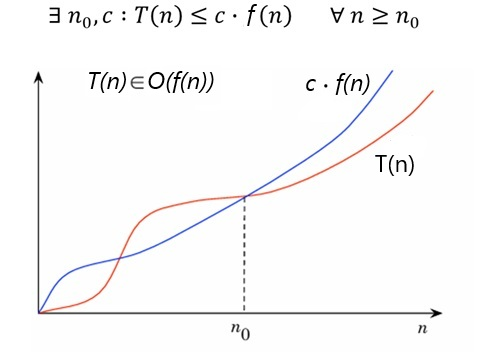
\includegraphics[width=0.6\textwidth]{immagini/1 - Complessità Computazionale/Ogrande.jpg}
	\caption{Rappresentazione grafica della notazione $O$ e del caso peggiore}
	\label{fig:1 - Complessità Computazionale:O-grande}
\end{figure}





\subsection{Notazione asintotica $\Omega$ e caso migliore}

Date due funzioni $T(n)$ e $f(n)$, si dice che $T(n) \in \Omega(f(n))$ se esistono costanti positive $c$ e $n_0$ tali che:

\[
0 \le c \cdot f(n) \le T(n) \quad \text{per ogni } n \ge n_0
\]

In altre parole, a partire da un certo valore di $n$, $f(n)$ rappresenta un limite inferiore asintotico per la crescita di $T(n)$.

Informalmente, $T(n) \in \Omega(f(n))$ se $T(n)$ \textbf{non cresce più lentamente di} $f(n)$.  
Approssimando la funzione $T(n)$ con $f(n)$ per $n > n_0$, si ottiene una \textbf{sottostima} di $T(n)$.

In informatica, il limite inferiore viene utilizzato per indicare il \textbf{caso migliore} di esecuzione di un algoritmo.  
Il tempo reale di esecuzione può variare a seconda dell'input, ma sostituendo $T(n)$ con una funzione semplice come $c \cdot f(n)$ che \textbf{sottostima} il tempo reale, otteniamo una stima valida almeno quanto il tempo minimo richiesto dall'algoritmo.

In figura \ref{fig:1 - Complessità Computazionale:Omega} è riportata la rappresentazione grafica di quanto detto.  
Sostituendo $T(n)$ con $c \cdot f(n)$ in questo contesto, stiamo considerando il \textbf{caso migliore} possibile.

\begin{figure}[h!]
	\centering
	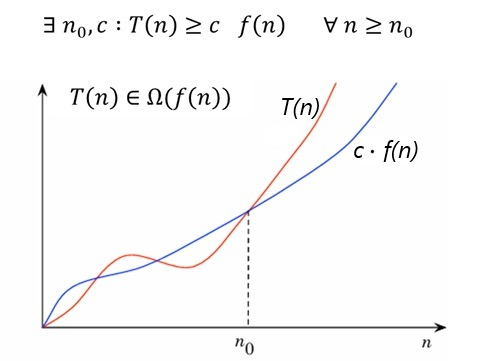
\includegraphics[width=0.6\textwidth]{immagini/1 - Complessità Computazionale/Sigmagrande.jpg}
	\caption{Rappresentazione grafica della notazione $\Omega$ e del caso migliore}
	\label{fig:1 - Complessità Computazionale:Omega}
\end{figure}


\subsection{Gerarchia delle complessità asintotiche}

Per avere un'idea chiara della velocità di crescita delle principali funzioni, possiamo organizzare le complessità asintotiche in una tabella.  
La tabella \ref{tab:1 - Complessità Computazionale:ordine_crescita} mostra le funzioni più comuni ordinate in \textbf{ordine crescente di crescita}, partendo dalle più lente fino a quelle che crescono più rapidamente.


\begin{table}[h!]
	\centering

	\renewcommand{\arraystretch}{1.5}

	\setlength{\tabcolsep}{12pt}
	\begin{tabular}{|c|c|}
		\hline
		\textbf{Ordine di crescita} & \textbf{Funzioni tipiche} \\
		\hline
		Costante & $O(1)$ \\
		\hline
		Logaritmica & $O(\log n)$ \\
		\hline
		Radicale & $O(\sqrt{n})$ \\
		\hline
		Lineare & $O(n)$ \\
		\hline
		Lineare-logaritmica & $O(n \log n)$ \\
		\hline
		Quadratica & $O(n^2)$ \\
		\hline
		Cubica & $O(n^3)$ \\
		\hline
		Polinomiale & $O(n^k),\ k>3$ \\
		\hline
		Esponenziale & $O(2^n), O(k^n)$ \\
		\hline
		Fattoriale & $O(n!)$ \\
		\hline
		Super-esponenziale & $O(n^n)$ \\
		\hline
	\end{tabular}
	\caption{Funzioni comuni ordinate per crescita asintotica}
	\label{tab:1 - Complessità Computazionale:ordine_crescita}
\end{table}



\subsection{Algebra della Notazione Asintotica}

Per semplificare il calcolo del costo computazionale asintotico degli algoritmi si possono sfruttare delle semplici regole che enunciamo senza riportarne la dimostrazione\footnote{Le regole che verranno riportate sono valide sia per il caso peggiore che per il caso migliore. Visto che nei problemi informatici siamo interessati quasi sempre al caso peggiore, riporteremo l'algebra della notazione asintotica \textbf{O}}.

\vspace{1cm}

\textbf{Prima regola: moltiplicazione per costante}  

Se esiste una funzione $T(n) \ge 0$ tale che:

\[
T(n) \in O(f(n)),
\]

allora, per ogni costante positiva $k > 0$, vale:

\[
k \cdot T(n) \in O(f(n)).
\]

Informalmente, possiamo enunciare questa regola dicendo che: \textbf{le costanti moltiplicative si possono ignorare.}


\vspace{1cm}
\textbf{Seconda regola: somma}  

Siano $T(n) \ge 0$ e $S(n) \ge 0$ due funzioni tali che:

\[
T(n) \in O(f(n)) \quad \text{e} \quad S(n) \in O(g(n)).
\]

Allora vale:

\[
T(n) + S(n) \in O(f(n) + g(n)) = O(\max(f(n), g(n))).
\]

In altre parole: \\
Se $f(n)$ cresce più velocemente di $g(n)$, allora $O(f(n) + g(n)) = O(f(n))$. \\
Se $g(n)$ cresce più velocemente di $f(n)$, allora $O(f(n) + g(n)) = O(g(n))$.

In termini ancora più semplici, possiamo affermare che in una somma si può \textbf{trascurare} il termine più piccolo.


\vspace{1cm}
\textbf{Terza regola: prodotto}  

Siano $T(n) \ge 0$ e $S(n) \ge 0$ due funzioni tali che:

\[
T(n) \in O(f(n)) \quad \text{e} \quad S(n) \in O(g(n)).
\]

Allora vale:

\[
T(n) \cdot S(n) \in O(f(n) \cdot g(n)).
\]

MOLTO informalmente, possiamo scrivere che:

\[
O(f(n)) \cdot O(g(n)) = O(f(n) \cdot g(n))
\]















\section{Complessità computazionale delle principali istruzioni}







\subsubsection{Operazioni elementari}

Tutte le operazioni elementari, ovvero:
\begin{itemize}
	\item assegnazione di una variabile,
	\item somma, sottrazione, moltiplicazione, divisione,
	\item confronto (<, >, ==, !=, ...),
	\item accesso all'elemento di un array con indice noto,
	\item input o output di una singola variabile,
\end{itemize}

hanno sempre complessità computazionale \textbf{O(1)}.

Consideriamo il seguente frammento di codice C++:

\begin{lstlisting}[language=C++]
	int a = 5;
	int b = 10;
	int c;
	int d;
	int e;
	
	if (a < b) {
		c = a + b;
		d = c * 2;
	} 
	else {
		c = a - b;
		d = c * 3;
		e = d + 1;
	}
\end{lstlisting}

Analizziamo il costo computazionale passo per passo:

\begin{itemize}
	\item \texttt{int a = 5;} $\rightarrow O(1)$  
	\item \texttt{int b = 10;} $\rightarrow O(1)$  
	\item \texttt{if (a < b)} $\rightarrow O(1)$ (un confronto tra due variabili)
\end{itemize}

A questo punto, il programma può entrare nel ramo \texttt{if} oppure nel ramo \texttt{else}:
\begin{itemize}
	\item Ramo \texttt{if}: due operazioni elementari  
	$\Rightarrow 2 \cdot O(1) = O(1)$
	\item Ramo \texttt{else}: tre operazioni elementari  
	$\Rightarrow 3 \cdot O(1) = O(1)$
\end{itemize}

Poiché i due rami sono alternativi (solo uno viene eseguito), si considera il ramo con complessità maggiore, in questo caso il ramo \texttt{else}.

La complessità totale del frammento è quindi:
\[
O(1) + O(1) + O(1) + O(1) = O(1)
\]

In conclusione, l’intero blocco ha complessità \textbf{costante}, indipendentemente dal valore delle variabili:  
il numero di operazioni non dipende da nessun parametro in ingresso.











\vspace{1cm}
\subsubsection{Complessità computazionale dei cicli}


\textbf{Ciclo for} \\

Consideriamo il seguente frammento di codice C++:

\begin{lstlisting}[language=C++]
	for (int i = 0; i < n; i++) {
		somma += i;
	}
\end{lstlisting}

Analizziamo il comportamento del ciclo:

\begin{itemize}
	\item L'inizializzazione \texttt{int i = 0} ha costo $O(1)$.
	\item La condizione \texttt{i < n} viene valutata $n + 1$ volte $\Rightarrow O(n + 1) = O(n)$.
	\item L'incremento \texttt{i++} viene eseguito $n$ volte $\Rightarrow O(n)$.
	\item Il corpo del ciclo \texttt{somma += i;} ha costo $O(1)$ per iterazione, quindi $n$ iterazioni $\Rightarrow O(n)$.
\end{itemize}

Sommando i costi:
\[
O(1) + O(n) + O(n) + O(n) = O(n)
\]

Il ciclo \texttt{for} ha dunque complessità complessiva \textbf{$O(n)$}, ovvero cresce linearmente con il numero di iterazioni.

\vspace{1cm}

\textbf{Ciclo while} \\

Il ciclo \texttt{while} ha un comportamento simile, ma il numero di iterazioni può dipendere da una condizione variabile.  
Esempio:

\begin{lstlisting}[language=C++]
	int i = 1;
	while (i < n) {
		i = i * 2;
	}
\end{lstlisting}

In questo caso, la variabile \texttt{i} raddoppia ad ogni iterazione, quindi il numero di iterazioni totali è pari al numero di volte in cui possiamo moltiplicare per 2 prima di superare $n$.

\[
i = 1 \Rightarrow 2 \Rightarrow 4 \Rightarrow 8 \Rightarrow \dots \Rightarrow n
\]

Il ciclo termina quando $2^k \ge n$, quindi $k = \log_2 n$.  
Di conseguenza, la complessità complessiva è:

\[
O(\log n)
\]

In generale, per un ciclo \texttt{while}, la complessità dipende dal numero di iterazioni necessarie affinché la condizione diventi falsa.


\vspace{1cm}
\subsubsection{Costrutti Misti e/o Annidati}

Quando i cicli sono combinati o condizionati tra loro, la complessità si calcola sommando o moltiplicando i costi dei vari blocchi, a seconda della struttura.

Esempio 1 — Cicli sequenziali:
\begin{lstlisting}[language=C++]
	for (int i = 0; i < n; i++) {
		// O(1)
	}
	for (int j = 0; j < n; j++) {
		// O(1)
	}
\end{lstlisting}

Le due sezioni non sono annidate ma consecutive, quindi:
\[
T(n) = O(n) + O(n) = O(n)
\]

Esempio 2 — Cicli annidati e condizione interna:
\begin{lstlisting}[language=C++]
	for (int i = 0; i < n; i++) {
		if (i % 2 == 0) {
			for (int j = 0; j < n; j++) {
				// O(1)
			}
		}
	}
\end{lstlisting}

Il ciclo interno si esegue solo per metà delle iterazioni esterne, ma l’ordine di grandezza resta invariato:
\[
T(n) = O\left(\frac{n}{2} \times n\right) = O(n^2)
\]










\vspace{1cm}
\subsubsection{Algoritmi con Procedure non ricorsive} 

La procedura generale che dev'essere seguita per il calcolo della complessità computazionale consiste nei seguenti passi:
\begin{itemize}
	\item si esamina il programma scendendo all'interno di ciascuna procedura o funzione fino ad individuare quella o quelle che non presentano chiamate ad altre procedure o funzioni al loro interno;
	
	\item per le procedure o funzioni che non contengono al loro interno chiamate ad altre procedure o funzioni, devono essere tenute presenti le considerazioni fatte fino ad ora e cioè applicare le regole sui singoli costrutti, in modo da determinare la complessità computazionale delle procedure o funzioni considerate come se fossero semplici blocchi di codice;
	
	\item determinata la complessità delle procedure/funzioni al punto precedente si passa a considerare invece la chiamata a queste ultime da parte di altre procedure/funzioni. Per ciascuna di tali procedure e funzioni viene calcolata la complessità computazionale, sostituendo a ciascuna chiamata di procedura o funzione la relativa complessità computazionale;
	
	\item si risale all'interno di questa pila di chiamate, ricordando la complessità computazionale calcolata ad ogni livello di risalita. Tale procedimento termina quando è stata calcolata la complessità di tutte le procedure e funzioni presenti nel programma principale;
	
	\item la complessità computazionale del \textit{main()} si calcola sostituendo a ciascuna chiamata di procedura o funzione la relativa complessità computazionale, calcolata secondo le regole descritte nei passi precedenti.
	
\end{itemize}


Ad esempio, si consideri il seguente programma:

\begin{lstlisting}[language=C++]
	#include <iostream>
	using namespace std;
	
	void stampaVettore(int A[], int n) {
		for (int i = 0; i < n; i++)
		cout << A[i] << " ";        // O(1)
	}
	
	int sommaVettore(int A[], int n) {
		int somma = 0;                   // O(1)
		for (int i = 0; i < n; i++)      // n iterazioni
		somma += A[i];               // O(1) per iterazione
		return somma;                    // O(1)
	}
	
	int main() {
		int n = 100;                     // O(1)
		int A[100];                      // O(1)
		
		for (int i = 0; i < n; i++)      // n iterazioni
		A[i] = i;                    // O(1) per iterazione
		
		stampaVettore(A, n);             // O(n)
		int risultato = sommaVettore(A, n); // O(n)
		
		cout << "Somma: " << risultato;  // O(1)
		return 0;
	}
\end{lstlisting}


\begin{enumerate}
	\item La funzione \texttt{stampaVettore()} contiene un ciclo \texttt{for} che scorre $n$ elementi, quindi:
	\[
	T_{\text{stampaVettore}}(n) = O(n)
	\]
	
	\item La funzione \texttt{sommaVettore()} ha anch’essa un ciclo su $n$ elementi, con operazioni elementari all’interno:
	\[
	T_{\text{sommaVettore}}(n) = O(n)
	\]
	
	\item La funzione \texttt{main()} esegue:
	\begin{itemize}
		\item Un ciclo \texttt{for} che inizializza un vettore di $n$ elementi → $O(n)$.
		\item Una chiamata a \texttt{stampaVettore()} → $O(n)$.
		\item Una chiamata a \texttt{sommaVettore()} → $O(n)$.
	\end{itemize}
	Applicando la regola della somma:
	\[
	T_{\text{main}}(n) = O(n) + O(n) + O(n) = O(n)
	\]
\end{enumerate}









\vspace{1cm}
\subsubsection{Algoritmi con Funzioni Ricorsive} 	

Per calcolare la complessità di un algoritmo ricorsivo non è possibile utilizzare le tecniche che abbiamo già analizzato, ma è necessario introdurre le \textbf{relazioni di ricorrenza}; esse descrivono una funzione nei termini del suo valore su input sempre più piccoli.




Ad esempio, consideriamo la funzione classica per calcolare la somma dei primi $n$ numeri:

\begin{lstlisting}[language=C++]
	#include <iostream>
	using namespace std;
	
	// Funzione ricorsiva
	int somma(int n) {
		if (n == 0) return 0;       // caso base O(1)
		return n + somma(n - 1);    // ricorsione
	}
	
	int main() {
		int n = 100;
		int risultato = somma(n);
		cout << "Somma: " << risultato;
		return 0;
	}
\end{lstlisting}

Analizzando la complessità, si nota che: 

\begin{itemize}
	\item La funzione \texttt{somma()} chiama se stessa una volta per ogni valore di $n$ fino al caso base:
	\[
	T(n) = T(n-1) + O(1)
	\]
	
	\item Espandendo passo passo:
	\[
	T(n) = O(1) + O(1) + \dots + O(1) \text{ (per n volte)} = O(n)
	\]
	
	\item La funzione \texttt{main()} esegue:
	\begin{itemize}
		\item Assegnazione di $n$ → O(1)
		\item Chiamata a \texttt{somma(n)} → O(n)
		\item Stampa del risultato → O(1)
	\end{itemize}
	
	Applicando la regola della somma:
	\[
	T_{\text{main}}(n) = O(1) + O(n) + O(1) = O(n)
	\]
\end{itemize}


\vspace{1cm}

Consideriamo un altro esempio: la versione ricorsiva della funzione di Fibonacci:

\begin{lstlisting}[language=C++]
	int fib(int n) {
		if (n <= 1) return n;
		return fib(n-1) + fib(n-2);
	}
\end{lstlisting}

Possiamo affermare che: 

\begin{itemize}
	\item La funzione chiama se stessa due volte per ogni valore di $n$ fino al caso base:
	\[
	T(n) = T(n-1) + T(n-2) + O(1)
	\]
	
	\item Questa ricorrenza cresce esponenzialmente, poiché ciascuna chiamata produce due nuove chiamate. Di conseguenza:
	\[
	T(n) = O(2^n)
	\]
\end{itemize}

\section{Esercizi di complessità computazionale}

\subsection{Esercizio 1}

Considera il seguente codice C++:

\begin{lstlisting}[language=C++]
	int a = 5, b = 10;
	int maxVal;
	
	if (a > b) {
		maxVal = a;
		b = b + 1;
	} else {
		maxVal = b;
		a = a + 1;
		b = b + 2;
	}
\end{lstlisting}

\textbf{Domanda:} Calcola la complessità computazionale totale di questo frammento di codice in termini di $O$.

\vspace{1cm}

\textbf{SOLUZIONE} \\

Analizziamo il frammento di codice riga per riga:

\begin{itemize}
	\item \texttt{int a = 5, b = 10;} $\rightarrow O(1)$ (assegnazione di variabili)
	\item \texttt{int maxVal;} $\rightarrow O(1)$ (assegnazione di variabile)
	\item \texttt{if (a > b)} $\rightarrow O(1)$ (confronto)
\end{itemize}

\textbf{Ramo vero:}
\begin{itemize}
	\item \texttt{maxVal = a;} $\rightarrow O(1)$
	\item \texttt{b = b + 1;} $\rightarrow O(1)$
\end{itemize}

\textbf{Ramo falso:}
\begin{itemize}
	\item \texttt{maxVal = b;} $\rightarrow O(1)$
	\item \texttt{a = a + 1;} $\rightarrow O(1)$
	\item \texttt{b = b + 2;} $\rightarrow O(1)$
\end{itemize}

\textbf{Somma complessiva:}  
Ogni ramo contiene un numero costante di operazioni $O(1)$.  
Applicando la regola della somma:

\[
T(n) = O(1) + O(1) + \max(O(1)+O(1),\ O(1)+O(1)+O(1)) = O(1)
\]

\textbf{Conclusione:}  
Il frammento di codice ha complessità totale $O(1)$.







\subsection{Esercizio 2}
Considera il seguente frammento di codice in C++:

\begin{lstlisting}[language=C++]
	int sum = 0;
	for (int i = 0; i < n; i++) {
		if (i % 2 == 0) {
			sum += i;
		} else {
			sum -= i;
		}
	}
\end{lstlisting}

\textbf{Domanda:}  
Determinare la complessità computazionale del frammento di codice sopra in termini di $n$.
Considerando un dispositivo capace di fare $10^8$ operazioni al secondo e considerando un input $n <10^4$, il tempo di esecuzione dell'algoritmo è inferiore a 1 secondo?


\vspace{1cm}

\textbf{SOLUZIONE} \\

Analizziamo ancora una volta il frammento di codice riga per riga:

\begin{itemize}
	
	\item \texttt{int sum = 0} $\rightarrow O(1)$
	
	\item Il ciclo \texttt{for(int i = 0; i < n; i++)} viene eseguito $n$ volte:
	
	quindi il ciclo contribuisce con $n \cdot T_{\text{interno}}$.
	
	\item All'interno del ciclo, abbiamo un \texttt{if-else}:
	\begin{itemize}
		\item Condizione \texttt{i \% 2 == 0} → O(1)
		\item Operazioni nel ramo vero \texttt{sum += i} → O(1)
		\item Operazioni nel ramo falso \texttt{sum -= i} → O(1)
	\end{itemize}
	Quindi ogni iterazione del ciclo ha complessità:
	\[
	T_{\text{iterazione}} = O(1) + O(1) = O(1)
	\]
	
	\item Moltiplicando per il numero di iterazioni:
	\[
	T_{\text{ciclo}} = n \cdot O(1) = O(n)
	\]
	
	\item Sommando tutte le parti del codice:
	\[
	T_{\text{totale}} = O(1) + O(n) = O(n)
	\]
\end{itemize}

\textbf{Conclusione:}  
La complessità complessiva del frammento di codice è $O(n)$.


\[
t_{\text{esecuzione}} \approx \frac{n}{10^8} < \frac{10^4}{10^8} = 10^{-4} \text{ secondi}
\]

\noindent
Poiché $10^{-4} \ll 1$, possiamo concludere che l'algoritmo termina molto prima di 1 secondo.






\subsection{Esercizio 3}

Consideriamo il seguente codice C++:

\begin{lstlisting}[language=C++]
	int sum = 0;
	for (int i = 0; i < n; i++) {
		for (int j = 0; j < m; j++) {
			sum += i + j;
		}
	}
\end{lstlisting}

\textbf{Domanda:}  
Determinare la complessità computazionale del frammento di codice sopra in termini di $n$.
Considerando un dispositivo capace di fare $10^8$ operazioni al secondo e considerando un input $n <10^4$ e $m < 10^3$, il tempo di esecuzione dell'algoritmo è inferiore a 1 secondo?

\textbf{Analisi della complessità:}

\begin{itemize}
	\item \texttt{int sum = 0} $\rightarrow O(1)$
	
	\item Il ciclo esterno \texttt{for(int i = 0; i < n; i++)} viene eseguito $n$ volte:
	quindi il ciclo contribuisce con $n \cdot T_{\text{interno}}$.
	
	\item Il ciclo interno \texttt{for(int j = 0; j < m; j++)} viene eseguito $m$ volte:
	quindi la complessità è $m \cdot T_{interno}$
	
	\item Nel ciclo interno abbiamo un'operazione elementare: $\texttt{sum += i+j} \rightarrow O(1)$.
	
	\item Applicando la regola del prodotto per i cicli annidati:
	\[
	T_{\text{ciclo}}(n,m) = n \cdot (m \cdot O(1)) = O(n \cdot m)
	\]
	
	\item Sommando l'assegnazione iniziale:
	\[
	T_{\text{totale}}(n,m) = O(1) + O(n \cdot m) = O(n \cdot m)
	\]
\end{itemize}

\textbf{Conclusione:}  
La complessità complessiva del frammento di codice è
\[
T(n,m) = O(n \cdot m)
\]


Il tempo di esecuzione è:
\[
t_{\text{esecuzione}} \approx \frac{n \cdot m}{10^8} < \frac{10^4 \cdot 10^3}{10^8} = \frac{10^7}{10^8} = 0.1 \text{ secondo}
\]

\noindent
Da cui ne deriva che il tempo di esecuzione è meno di 1 secondo (ma non di molto).

